\section{Architecture}
\label{sec:method}

\subsection{Problem statement}

An instance is a state $s$ and a set of questions $Q = \{q_1,\dots,q_m\}$.
Each question $q_i$ carries instructions and an option set $O_i =
\{o_{i,1},\dots,o_{i,K_i}\}$, with $K_i$ varying freely across questions in
the same call. The model must return, for every question, a distribution
over that question's own options:
\[
  p(o_{i,j} \mid s, q_i), \qquad \sum_{j=1}^{K_i} p(o_{i,j}\mid s,q_i) = 1 .
\]
Two properties are required. The cost must be sublinear in $m$, since a
production router asks ten questions where a benchmark asks one. And
$p(\cdot)$ must be a usable probability, because the operational decision
is a threshold on it.

\subsection{Packing}

We write the state once, then each question and its options after it, as a
single token sequence (Figure~\ref{fig:packing}); which positions may
then attend to which is Figure~\ref{fig:mask}. Each option is followed
(or preceded, depending on backbone) by a \emph{marker} token, and the
model's output for that option is read at the marker position.

Formally, the packed sequence carries a block assignment $b(t) \in
\{0,1,\dots,m\}$ for each token position $t$, where block $0$ is the shared
state prefix and block $i$ holds question $q_i$ with its options.

\begin{figure}[t]
\centering
\footnotesize
\setlength{\tabcolsep}{3pt}
\begin{tabular}{|l|l|l|l|}
\hline
\multicolumn{1}{|c|}{\textbf{block 0: shared state}} &
\multicolumn{1}{c|}{\textbf{block 1}} &
\multicolumn{1}{c|}{\textbf{block 2}} &
\multicolumn{1}{c|}{\textbf{block 3}} \\
\hline
\emph{``I need a refill, and} & \texttt{intent?} & \texttt{clinical?} & \texttt{urgent?} \\
\emph{are you open Sunday?''} & \texttt{refill}~$\bullet$ & \texttt{no}~$\bullet$ & \texttt{low}~$\bullet$ \\
 & \texttt{hours}~$\bullet$ & \texttt{yes}~$\bullet$ & \texttt{high}~$\bullet$ \\
\hline
\end{tabular}
\caption{Packing. The state is encoded once. Each option ends in a marker
$\bullet$ where the score is read. Every block attends to block 0 and to
itself; no block attends to another. Asking question 3 therefore cannot
change the answer to question 1.}
\label{fig:packing}
\end{figure}

\subsection{Block-diagonal attention}

Let $A(t,u) \in \{0,1\}$ indicate whether query position $t$ may attend to
key position $u$. We impose
\begin{equation}
  A(t,u) \;=\; \underbrace{\mathbb{1}\big[\, b(u) = 0 \;\lor\; b(u) = b(t)
  \,\big]}_{\text{our rule}} \cdot \underbrace{C(t,u)}_{\text{backbone's own}},
  \label{eq:mask}
\end{equation}
where $C(t,u) = 1$ for a bidirectional encoder and $C(t,u) = \mathbb{1}[u
\le t]$ for a causal decoder. Both factors are indicators, so the product
is the conjunction.

The first factor is what makes the shared prefix legitimate: every question
sees the full state. The second is what makes the result well defined.
Without it, question 2 attends to question 1 and an answer becomes a
function of which other questions happened to be asked in the same call.
On a causal backbone the state already precedes every question, so the
rule's only remaining work is isolating question blocks from each other.
Figure~\ref{fig:mask} shows both cases.

\begin{figure}[t]
\centering
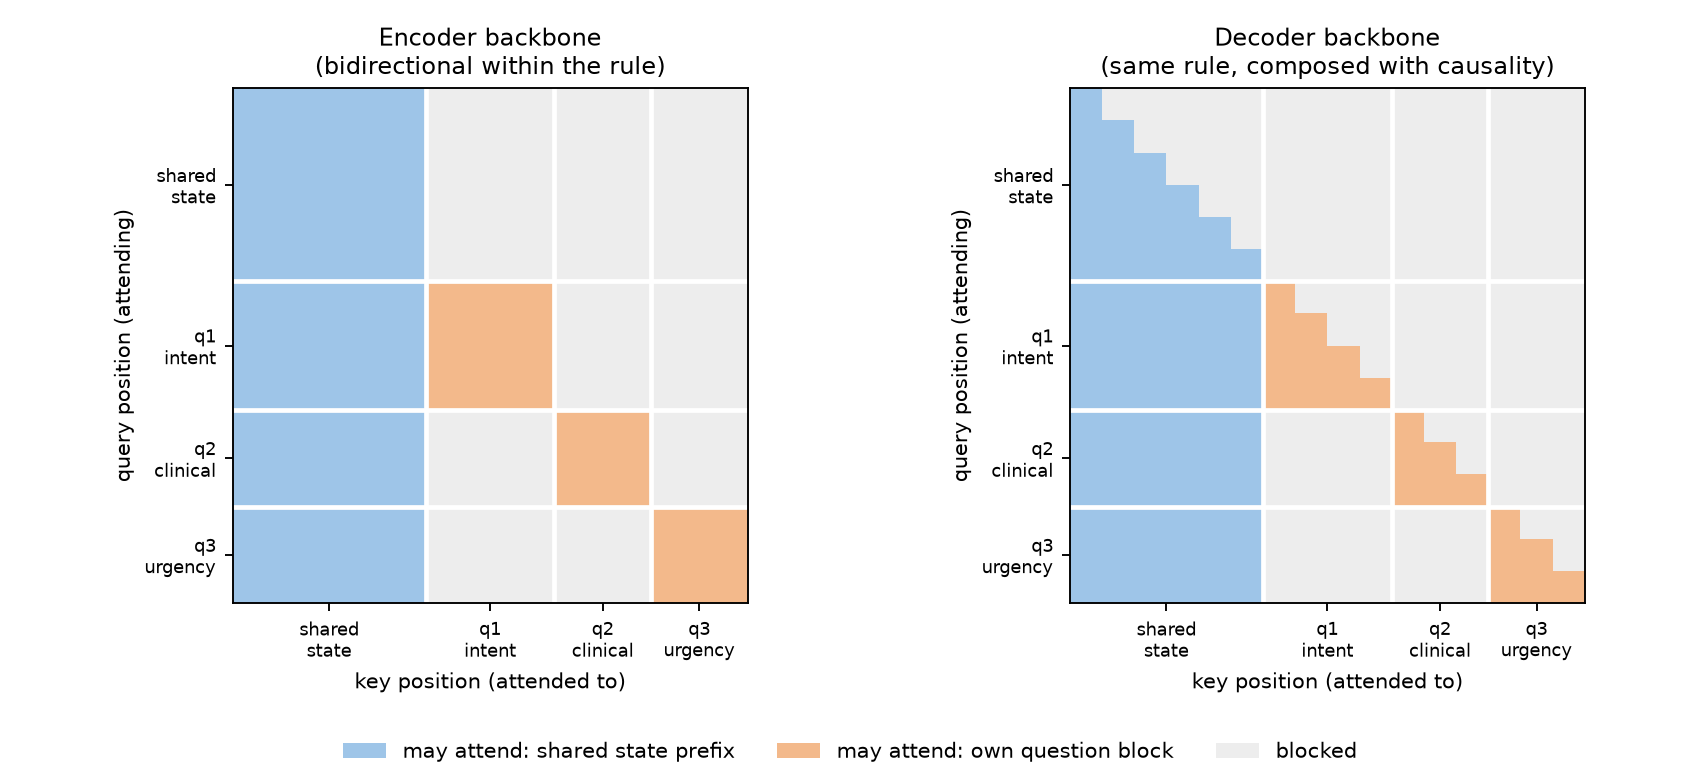
\includegraphics[width=\textwidth]{figures/attention_mask.png}
\caption{The mask of Eq.~\ref{eq:mask} for a packed sequence with a shared
state and three questions. Blue is attention to the shared prefix, orange
is attention within a question's own block, grey is blocked. No question
can see another, so its answer does not depend on what else was asked.
Right: the same rule composed with causality on a decoder backbone.}
\label{fig:mask}
\end{figure}

\paragraph{Memory.} The mask is $O(n^2)$ in sequence length, which is the
usual attention cost and not specific to this design, but it does bound
how many questions fit in one call. At our 2048-token budget a
ten-question router with 24 options packs comfortably; a 151-option menu
rendered with long descriptions does not, and the implementation degrades
by subsampling the menu (always keeping the gold) rather than failing.

\subsection{Readout and grouped normalisation}

Let $h_t$ be the final hidden state at marker position $t$, and let
$\mathcal{M}_i$ be the marker positions of question $q_i$. A scalar score
is produced per option. For an encoder backbone this is a shared linear
scorer, $z_t = w^\top h_t + b$. For a decoder backbone it is the difference
of two vocabulary logits at the marker,
\begin{equation}
  z_t = \big[W_{\text{lm}} h_t\big]_{\texttt{yes}} - \big[W_{\text{lm}}
  h_t\big]_{\texttt{no}},
  \label{eq:yesno}
\end{equation}
optionally plus a residual head $g(h_t)$ initialised to zero, so that
training begins at exactly the untrained readout.

Because $K_i$ differs across questions packed into one sequence, scores are
normalised \emph{within} each question rather than globally:
\begin{equation}
  p(o_{i,j}\mid s,q_i) = \frac{\exp(z_{t_{i,j}})}{\sum_{t\in\mathcal{M}_i}
  \exp(z_t)} .
  \label{eq:grouped}
\end{equation}
This is a segmented softmax over a ragged partition of the flat marker
array. Writing $y_i$ for the index of the gold option of question $q_i$,
and $\mathcal{A}$ for the questions this example actually answers (a row
may supervise only some of them), the loss is
\begin{equation}
  \mathcal{L} \;=\; -\frac{1}{|\mathcal{A}|}
  \sum_{i \in \mathcal{A}} \log p\big(o_{i,y_i} \mid s, q_i\big).
  \label{eq:loss}
\end{equation}

\paragraph{A worked example.} Suppose one packed sequence holds $q_1$ with
$K_1{=}3$ and $q_2$ with $K_2{=}2$, so the flat marker array has five
entries with scores $z = [2.0,\,1.0,\,0.5,\;\;0.2,\,1.4]$ and the
partition $\mathcal{M}_1 = \{1,2,3\}$, $\mathcal{M}_2 = \{4,5\}$. A global
softmax over all five would make $q_1$'s options compete with $q_2$'s,
which is meaningless. Grouped, we get $p_1 \approx [0.63, 0.23, 0.14]$ and
$p_2 \approx [0.23, 0.77]$, each summing to one. If the golds are
$y_1{=}1$ and $y_2{=}2$, then $\mathcal{L} = -\tfrac{1}{2}(\log 0.63 +
\log 0.77) \approx 0.36$.

\begin{algorithm}[t]
\caption{Forward pass for one packed instance}
\label{alg:forward}
\begin{algorithmic}[1]
\Require state $s$, questions $Q=\{q_i\}$ with option sets $O_i$
\State $x, b, \mathcal{M} \gets \textproc{Pack}(s, Q)$
  \Comment{tokens, block ids, marker positions}
\State $A \gets$ mask from Eq.~\ref{eq:mask} using $b$ and backbone
  constraint $C$
\State $H \gets \textproc{Backbone}(x, A)$
  \Comment{one forward pass, all questions}
\State $z \gets \textproc{Score}(H[\mathcal{M}])$
  \Comment{linear, or Eq.~\ref{eq:yesno} for a decoder}
\ForAll{questions $q_i$}
  \State $p_i \gets \textproc{Softmax}(z[\mathcal{M}_i])$
    \Comment{grouped, Eq.~\ref{eq:grouped}}
\EndFor
\State \Return $\{p_i\}$
\end{algorithmic}
\end{algorithm}

\subsection{Rendering the three primitives}

How an option is written to the sequence matters more than one would
expect, and \S\ref{sec:res-architecture} quantifies it. The rules we
converged on:

\begin{itemize}[leftmargin=1.4em,itemsep=0.25em]
  \item \choice{}: label and description both, since both carry meaning.
    Where the two are identical, as in multiple-choice tasks whose
    option \emph{is} its own description, they are collapsed, or every
    option is emitted twice.
  \item \score{}: the level description alone. Rendering a level as
    \texttt{"0: very negative: \ldots"} asks the model to score a bare
    index.
  \item \noul{}: bare polarity, \texttt{no}/\texttt{yes}, and \emph{not}
    the descriptions. A \noul{}'s two descriptions necessarily restate one
    judgement from opposite sides, so scoring both measures their overlap.
    Measured, this costs AUROC $0.63$ against $0.712$
    (\S\ref{sec:res-architecture}).
\end{itemize}

\subsection{Cost}

The state is encoded once regardless of $m$, so the marginal cost of a
question is its own options. Measured on the ten-question router with a
1.7B backbone, median latency per state is $69$\,ms for one question and
$74$\,ms for ten: \textbf{ten questions cost 6\% more than one}. The
reference API shows the same signature, $392$\,ms against $407$\,ms, which
is the evidence that it shares this design.

\paragraph{On the two sets of latency numbers in this paper.} The figures
here ($69$ and $74$\,ms) were taken while a training run shared the GPU;
those in \S\ref{sec:res-latency} ($37.7$ to $55.9$\,ms) were taken under
lighter load. Absolute values are therefore not comparable across the two
sections and only the within-section ratios are meaningful. We report both
rather than the flattering one, and neither is a throughput measurement:
everything here is batch size 1, which is the interactive case. Sustained
throughput under load is not measured in this work.
